\section{Overview}

In this section, we introduce the overall structure of JSSET and the outline of
this paper. Figure~\ref{fig:overview} depicts the overall structure of JSSET.
It mechanizes to extract syntax and semantics of ECMAScript using
two main module; the \textit{parser generator} and the \textit{algorithm compiler}.
If first extracts information via the spec extractor.
ECMAScript specifications are provided as a readable HTML file.
Thus, we develop the spec extractor in JavaScript to automatically
extract their contents.

\begin{figure}
  \centering
  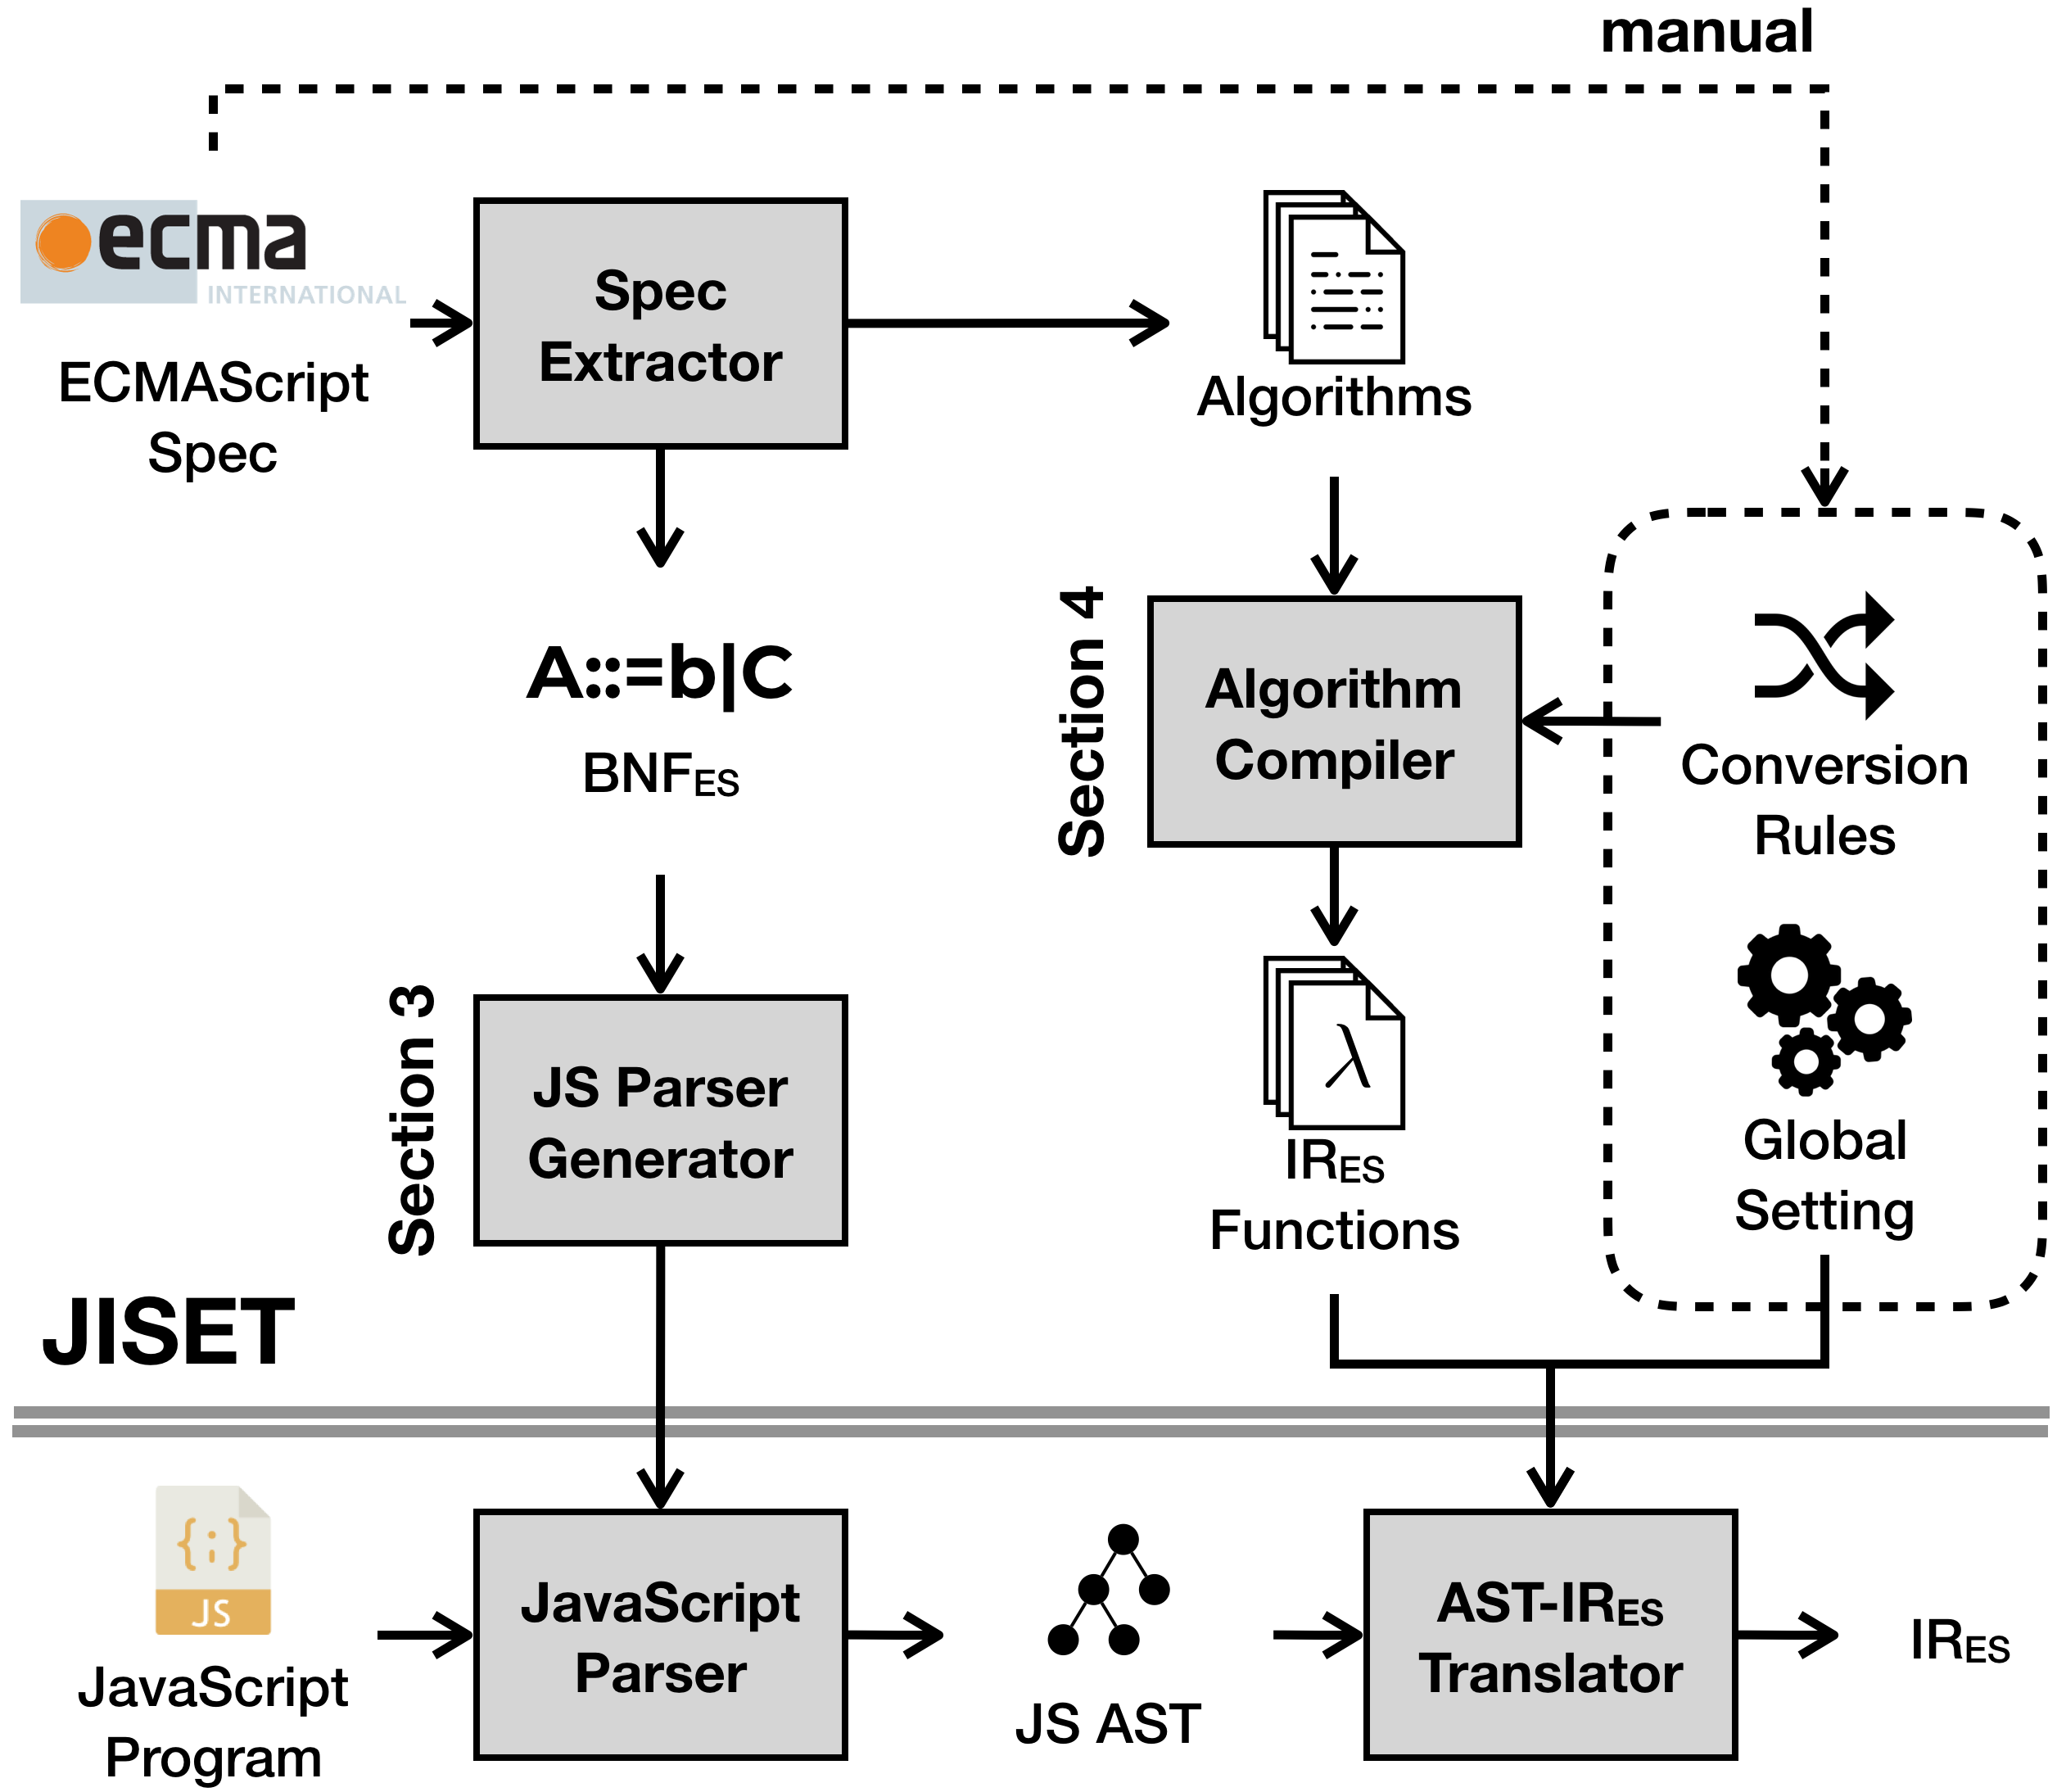
\includegraphics[width=0.5\textwidth]{img/overview.png}
  \caption{Overall structure of JavaScript Semantics Extraction Toolchain (JSSET)}
  \label{fig:overview}
\end{figure}

ECMAScript specifications describe their lexical and syntactic grammars
based on their own extension of Backus-Naur Form (BNF).
We call it as \( \bnfes \), BNF for ECMAScript specifications.
It supports additional notations for parametric productions, conditional
right-hand sides, optional symbols, positive/negative lookaheads,
exclusive symbols, and no line-terminator symbols. We first formally define
\( \bnfes \) and build the spec extractor to extract grammars written in \( \bnfes \).
Then, we carefully construct the \textit{parser generator} for them by extending
the Scala parser combinators. Moreover, we propose \textit{lookahead parsers}
to parse \( \bnfes \) for correct and fast parsing.
A lookahead parser keeps track of its lookahead, which is the set of
possible next tokens. With lookahead parsers,
the parser generator automatically generate parsers for ECMAScript grammars.
The generated parsers are readable and one-to-one corresponds to each
grammar components.
For example, Firugre~\ref{fig:array-literal-es} is ArrayLiteral production in
ECMAScript 2019 specification and Figure~\ref{fig:array-literal-parser}
is the generated parser of the algorithm written in Scala.
In the first right-hand side, the optional \( Elision \) token
is represented as \( \code{opt(Elision)} \).
The parametric non-terminal \( ElementList \) with arguments \( Yield \)
and \( Await \) is represented as \( \code{ElementList(Yield, Await)} \).

\begin{figure}
  \centering
  \begin{subfigure}[t]{0.4\textwidth}
    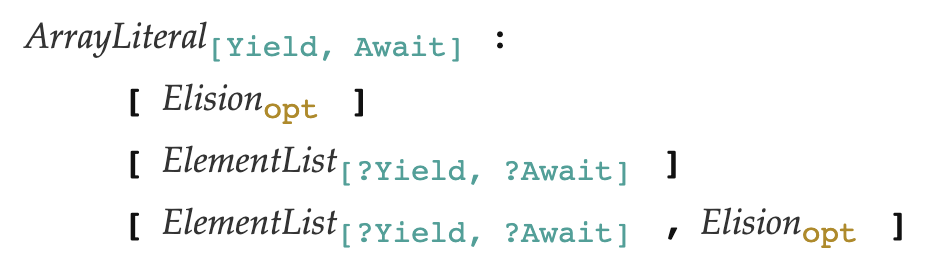
\includegraphics[width=\textwidth]{img/array_literal.png}
    \caption{ArrayLiteral production in ECMAScript 2019 specification.}
    \label{fig:array-literal-es}
  \end{subfigure}
  \begin{subfigure}[t]{0.5\textwidth}
    \begin{lstlisting}[style=myScalastyle]
type P[T] = List[Boolean] => LAParser[T]
lazy val ArrayLiteral: P[ArrayLiteral] = memo {
  case List(Yield, Await) =>
  "[" ~ opt(Elision) ~ "]" ^^ ArrayLiteral0 |
  "[" ~ ElementList(Yield, Await) ~ "]" ^^ ArrayLiteral1 |
  "[" ~ ElementList(Yield, Await) ~ "," ~ opt(Elision) ~ "]" ^^ ArrayLiteral2
}
    \end{lstlisting}
    \caption{The generated parser for ArrayLiteral production.}
    \label{fig:array-literal-parser}
  \end{subfigure}
  \caption{ArrayLiteral grammar production in ECMAScript 2019.}
  \label{fig:array-literal}
\end{figure}

The semantics in ECMAScript specifications are described as
abstract algorithms. They are written in structured natural languages
with ordered steps and tagged tokens. For example, Figure~\ref{fig:to-primitive-es}
is an example abstract algorithm for \( \code{ToPrimitive} \) in
ECMAScript 2019. The spec extractor extracts each abstract algorithm
with HTML tags because we utilize tag information to discriminate
different kinds of tokens. Then, the \textit{algorithm compiler} converts
given abstract algorithms into funcitons of our core language \( \ires \).
The compilation is dependent on manually defined conversion rules
that consists of two parts; parsing rules and mapping from each rule into \( \ires \)
component. We carefully define \( \ires \) to directly match instructions with
the corresponding algorithm steps. For example, Figure~\ref{fig:to-primitive-ires}
describes the generated \( \ires \) function for the \( \code{ToPrimitive} \)
algorithm. Each instruction of the generated \( \ires \) function
is easily matched with the corresponding algorithm step
and also they have similar silhouettes.

\begin{figure*}[t]
  \centering
  \begin{subfigure}{0.4\textwidth}
    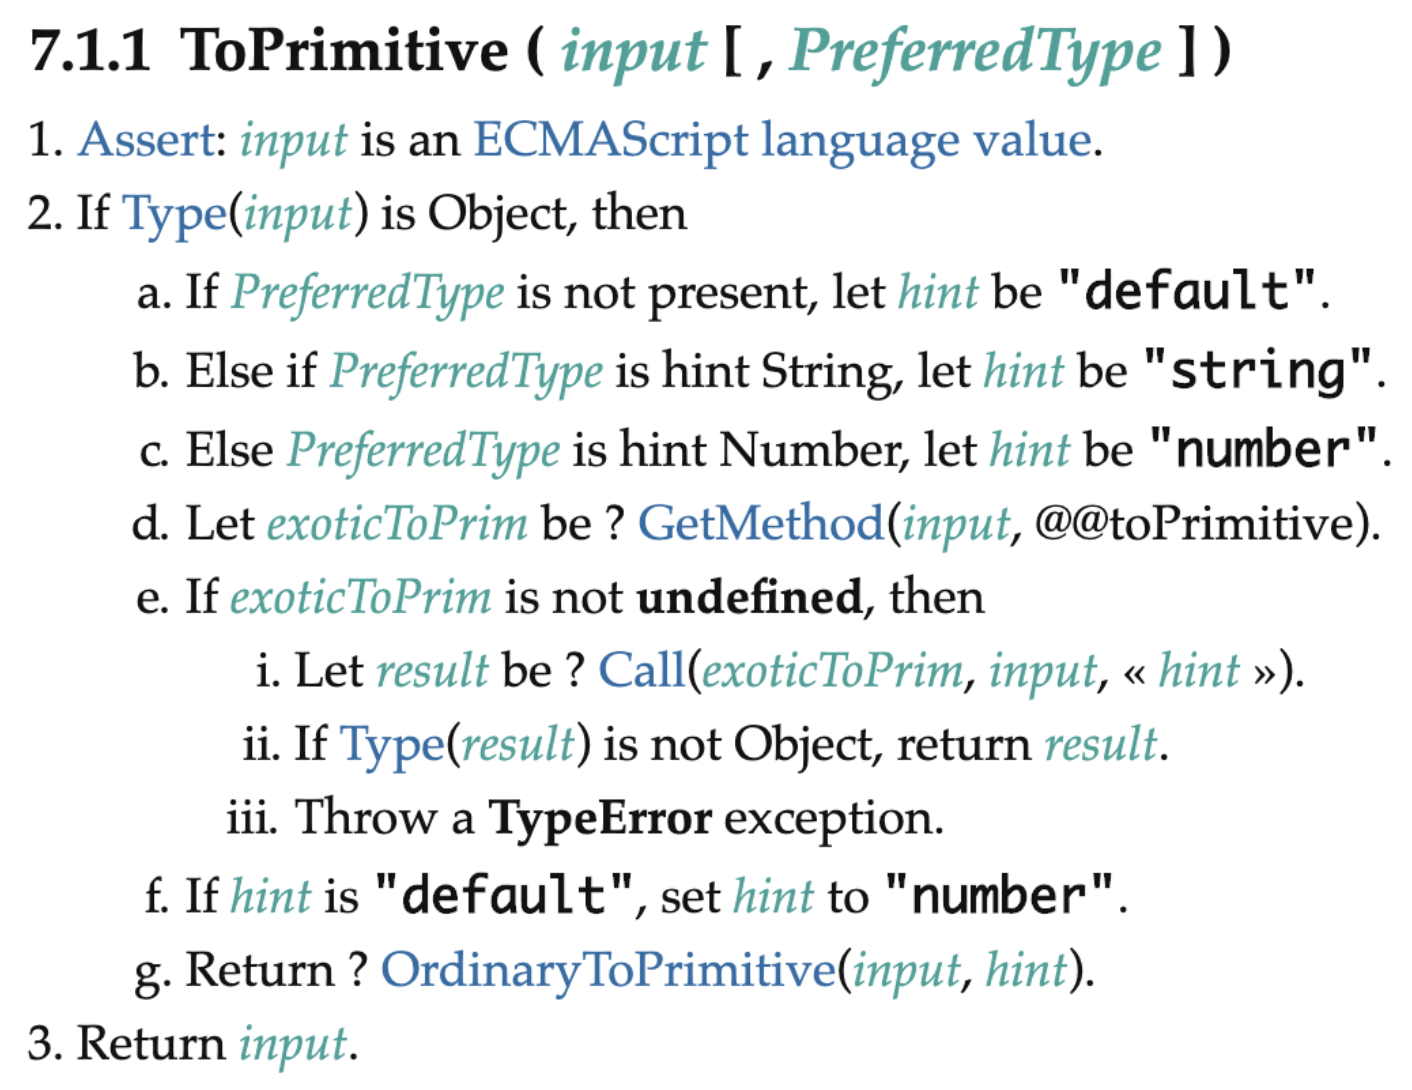
\includegraphics[width=\textwidth]{img/to_primitive.png}
    \subcaption{\( \code{ToPrimitive} \) abstract algorithm in ES2019.}
    \label{fig:to-primitive-es}
  \end{subfigure}
  \qquad
  \begin{subfigure}{0.48\textwidth}
    \begin{lstlisting}[style=ires]
"ToPrimitive" (input, PreferredType) => {
  if (= (Type input) "Object") {
    if (= PreferredType absent) let hint = "default"
    else if (= PreferredType "String") let hint = "string"
    else let hint = "number"
    let exoticToPrim = ? (GetMethod input SYMBOL_toPrimitive)
    if (! (= exoticToPrim undefined)) {
      let result = ? (Call exoticToPrim input (new [hint]))
      if (! (= (Type result) "Object")) return result
      return (Throw INTRINSIC_TypeErrorPrototype)
    }
    if (= hint "default") hint = "number"
    return ? (OrdinaryToPrimitive input hint)
  }
  return input
}
    \end{lstlisting}
    \subcaption{The \( \ires \) funciton for \( \code{ToPrimitive} \)
    abstract algorithm.}
    \label{fig:to-primitive-ires}
  \end{subfigure}
  \caption{\( \code{ToPrimitive} \) abstract algorithms
  and its generated core program.}
  \label{fig:to-primitive}
\end{figure*}

Finally, the generated \( \ires \) functions with mannual initial settings
are applied into the \( \ires \) interpreter. We could parse a
given JavaScript program using the generated JavaScript parser
to get the abstract syntax tree (AST). Then, the \( \ires \) interpreter
evaluates the given AST and provides evaluation results.

From now, we describe the detailed techniques of JSSET.
Section 3 formallly defines \( \bnfes \) and how to automatically
generate parsers from given \( \bnfes \) using lookahead parsers.
Section 4 explains abstract algorithms with tagged tokens
and how to compile them into \( \ires \) functions based on
given conversion rules. Section 5 describes the implemented details
about initial settings to evaluate JavaScript programs. Section 6
discusses the effectiveness of JSSET with four research questions.
Section 7 discusses related work and Section 8 concludes.
